\section{\Large{Specifications}}
\begin{enumerate}[label=\arabic*.]

%%%%%%%%%%%%%%%%%%%%%%%%%%%%%%%%%%%%%%%
    \item {\large{Example}}
    \begin{enumerate}[label*={\arabic*.},ref=\theenumi.\arabic*]
    \setlength{\itemindent}{0.5cm}
        \item
            \begin{table}[H]
            \center
                \begin{tabular}{m{1.4cm} m{5.5cm}}
                \toprule
                \# of Req. & Description\\
                \midrule
                Req 1.1. & The user must log in to their own account, which contains their personal information.\\\\
                Req 1.5. & Alternatively, users can utilize an external ID, like a Google or Apple ID, to conveniently sign in without having to register.\\\\
                \bottomrule
                \end{tabular}
            \end{table}
            
                \begin{figure}[ht]
                    \begin{center}
                    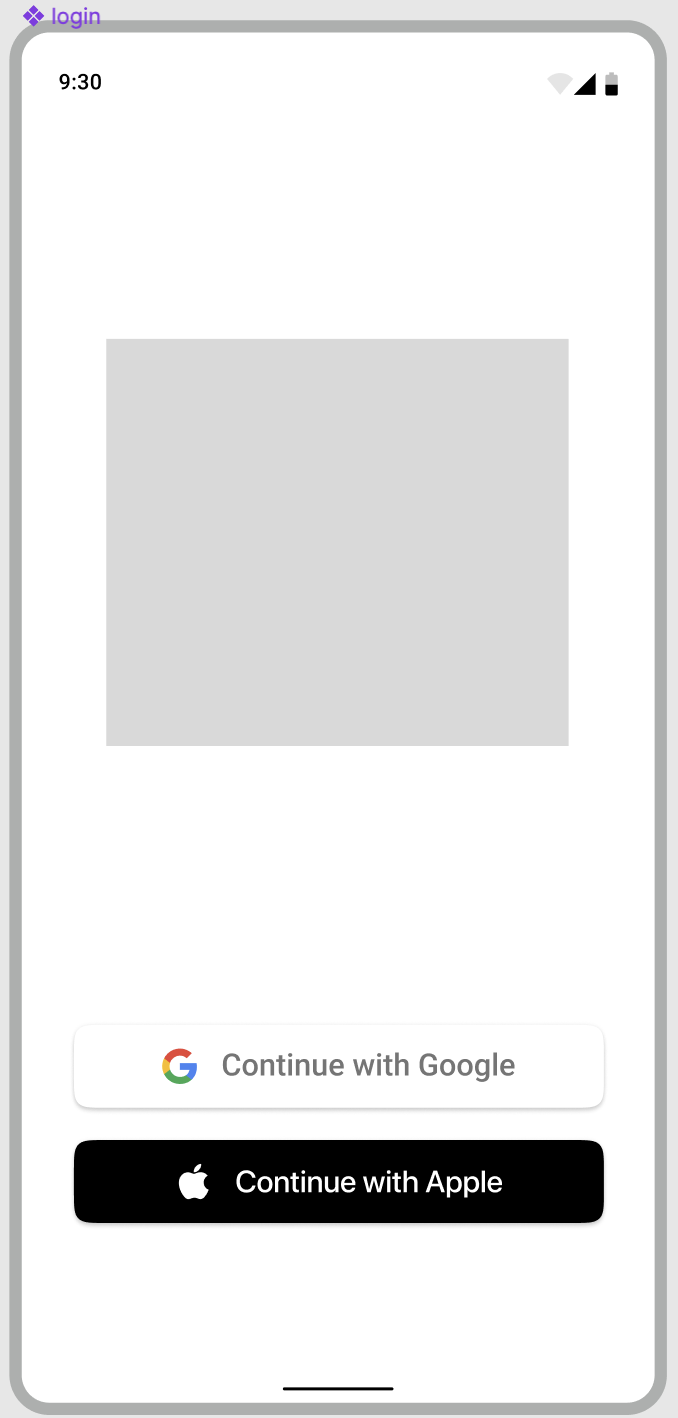
\includegraphics[width=3.5cm]{imgs/specification/login_page.png}
                    \caption{Login page}
                    \renewcommand{\thefigure}{\thesubsection.\arabic{figure}}
                    \end{center}
                \end{figure}
            There are two buttons on login page, 'Continue with Google' and 'Continue with Apple'. When the user click the button, login is success and move to the main page.\\\\

        \item
            \begin{table}[H]
            \center
                \begin{tabular}{m{1.4cm} m{5.5cm}}
                \toprule
                \# of Req. & Description\\
                \midrule
                Req 1.1. & The user must log in to their own account, which contains their personal information.\\\\
                \bottomrule
                \end{tabular}
            \end{table}
            
            \begin{center}
                \begin{figure}[ht]
                    \begin{center}
                    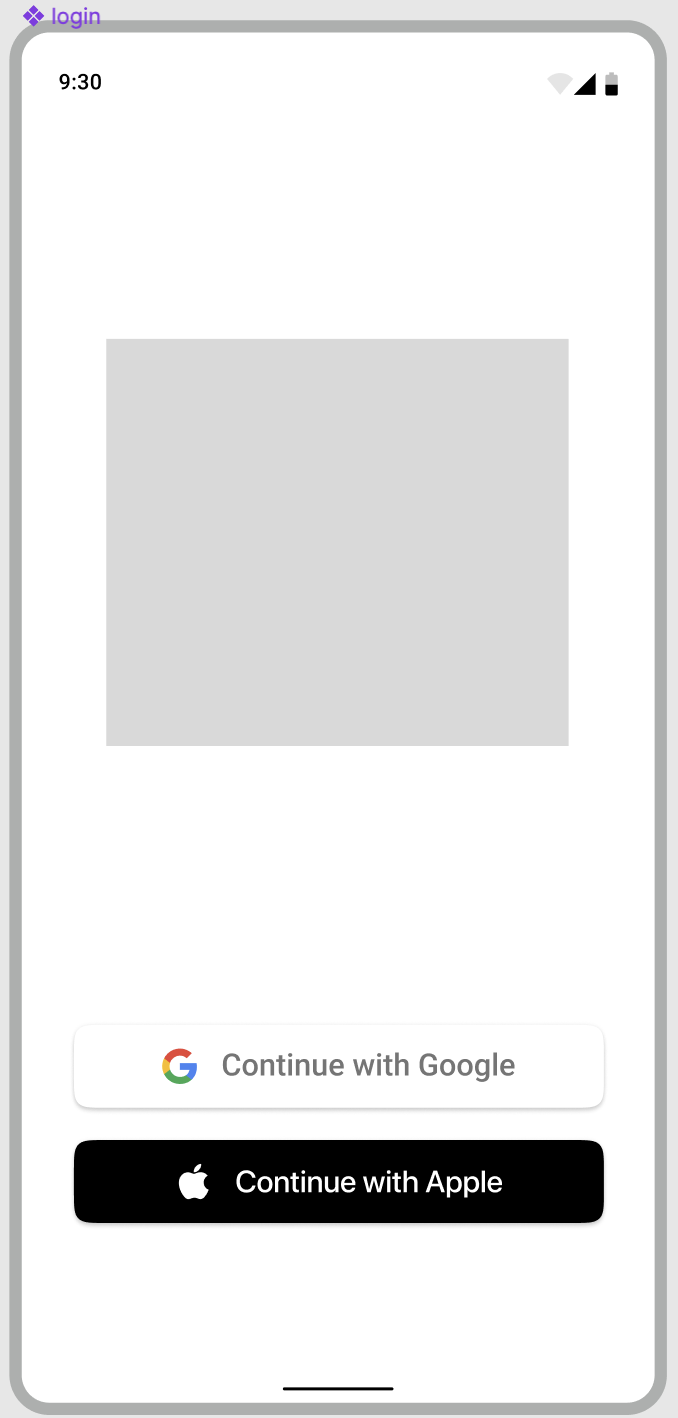
\includegraphics[width=3.5cm]{imgs/specification/login_page.png}
                    \caption{Login page}
                    \renewcommand{\thefigure}{\thesubsection.\arabic{figure}}
                    \end{center}
                \end{figure}
            \end{center}
            There are two buttons on login page, 'Continue with Google' and 'Continue with Apple'. When the user click the button, login is success and move to the main page.\\\\
    \end{enumerate}
%%%%%%%%%%%%%%%%%%%%%%%%%%%%%%%%%%%%%%%
    
    \item {\large{Login Page}}
    \begin{enumerate}[label=\alph*]
        \item There are two buttons on login page, 'Continue with Google' and 'Continue with Apple'. When the user click the button, login is success and move to the main page.
        \item On the main page, there is 'plus' button which makes the page move to 'add Device' page. The user can add Matter devices through QR code on this page. There is also the button, 'Connect without the QR code'. 
    \end{enumerate}
    \item {\large{Log Page}}
    \begin{enumerate}[label=\alph*]
        \item At the Bottom of the page, there is the menu named 'Log'. When the user click the 'Log' button, He/She can see their routine logs. This application records and stores information such as the user's location, posture, and sensors by time period 
    \end{enumerate}
    \item {\large{Routine Page}}\\
    Here you can view all plans that the user has set. You can click on them to view the status, or click the start button to start them manually. If you need to create a new plan yourself, you can also click the plus sign in the lower right corner to customize the plan by setting triggers and activities.\\
    \begin{enumerate}[label=\alph*]
        \item Create new routine\\
            Click the plus sign in the lower right corner of the page to create your own routine. Enter the name of the desired routine in the pop-up window and click "Add" to enter the routine setting page.\\

            
        \item Routine Setting Page\\
            Click the set routine page to adjust the set routine. In the settings page, you can modify the name of the routine, share the routine, and delete the routine. On the right side you can select the switch for this routine. Below is the setting of trigger type. Different conditions can be selected according to different triggers. After selecting, click the check mark in the upper right corner to save.\\
            \begin{enumerate}
                \item  Location Trigger Settings\\
                    To do.\\
                \item  Posture Trigger Settings\\
                    After clicking on the pose trigger settings, first select the camera you want to use, and then you can select the action you want to trigger. There is now a choice of three recognized postures, sitting, standing and lying down. You can choose to perform the following actions after the camera recognizes which posture it is. Such as turning on a light or turning on a switch. The actions performed can also be set by yourself.\\
                \item  Voice Assistant Trigger Settings\\
                    After clicking the voice assistant trigger setting, you can choose the voice command when you want to execute the command. Different triggers can be triggered based on the recognized voice command.\\
                \item  Schedule Trigger Settings\\
                    After clicking on the scheduled trigger setting, you can select the time to be set in the prompt box below, and the trigger will be automatically executed after this time.\\
            \end{enumerate}
            
        \item behavior routine
        \begin{enumerate}
            \item It was implemented to adjust the intensity of the light through the light-on motion bulk sldier, and the switch on/off function was implemented\\
            

            \item In the routine item, a todo list was implemented for each trigger, such as construct detect and schedule, and actions to be performed for each todo were implemented. Switch off time delay
        \end{enumerate}
        \item setting
            \begin{enumerate}
            \item The on/off button that alerts you when the routine is started by a particular trigger has implemented a button that can be turned on and off according to touch, with the 'push alarm on route starts' written in the notification-shaped column\\

            \item Each user created a Backup/Restore column to back up and import routines, and Backup routes implemented it with the download shape and Restore routes with the upload shape\\

            \item username in a pencil shape so that intuitively see that it can be modified, and created a logout button at the bottom and implemented it so that easily change my account\\

            \item Implemented 'Delete all settings' with trash bin shape to delete all settings
    \end{enumerate}
\end{enumerate}
\end{enumerate}